

%\usepackage{tikz}
\usetikzlibrary{calc}


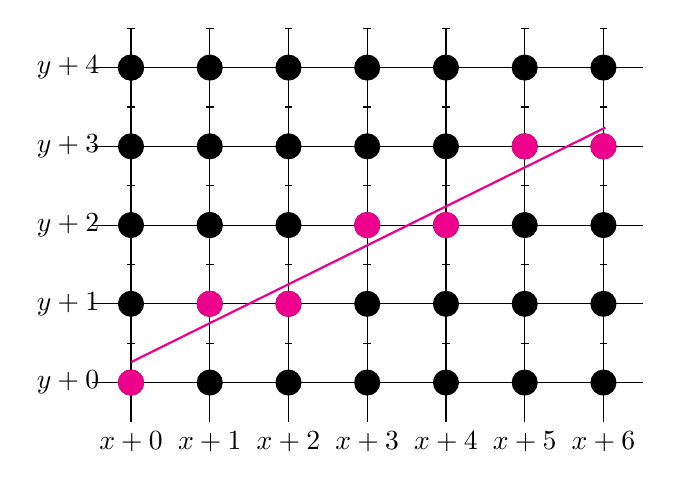
\begin{tikzpicture}
	\begin{scope}
		
\tikzset{dot/.style={fill=black,circle}}

%\foreach\l[count=\y] in {E,...,A}
\foreach \y in {0,1,...,4}
{
\draw (0.5,\y+1) -- (7.5,\y+1);
\node at (0.2,\y+1){$y + \y$};
}

\foreach \x in {0,1,...,6}
{
\draw (\x+1,0.5) -- (\x+1,5.5);
\node at (\x+1, 0.25){$x + \x$};
}

\foreach \x in {1,2,...,7}
{
	\foreach \y in {1,2,...,5}
	{
		\node[dot] at (\x,\y){};
		\draw(\x-0.05,\y+0.5) --(\x+0.05,\y+0.5);
	}
}


\node(p1)[dot] at (1,5){};
\node(p2)[dot] at (2,3){};

% the actual line
\node(st) at (0.88,1.2){};
\node(end) at (7.15,4.3){};
\draw [magenta, thick] (st) -- (end);

% draw its Bresenham points
\node[dot,magenta] at (1,1){};
\node[dot,magenta] at (2,2){};
\node[dot,magenta] at (3,2){};
\node[dot,magenta] at (4,3){};
\node[dot,magenta] at (5,3){};
\node[dot,magenta] at (6,4){};
\node[dot,magenta] at (7,4){};

	\end{scope}
\end{tikzpicture}
